\documentclass{article}

\def\ParSkip{} 
% Packages
\usepackage{amssymb,amsmath,amsthm,bbm}
\usepackage{verbatim,float,url,dsfont}
\usepackage{graphicx,subfigure,psfrag}
\usepackage{algorithm,algorithmic}
\usepackage{mathtools,enumitem}
\usepackage{multirow}
\usepackage{ragged2e}
\usepackage{xr-hyper}
\usepackage{array}

\usepackage[colorlinks=true,citecolor=blue,urlcolor=blue,linkcolor=blue]{hyperref}
\usepackage[margin=1in]{geometry}
\usepackage[round]{natbib}

\usepackage[utf8]{inputenc} % allow utf-8 input
\usepackage[T1]{fontenc}    % use 8-bit T1 fonts
\usepackage{booktabs}       % professional-quality tables
\usepackage{nicefrac}         % compact symbols for 1/2, etc.
\usepackage{microtype}      % microtypography

\ifdefined\TimesFont 
\usepackage{times} % use times font
\fi

\ifdefined\ParSkip 
\usepackage{parskip} % use par skip
\fi

% Theorems and such
\newtheorem{theorem}{Theorem}
\newtheorem{lemma}{Lemma}
\newtheorem{corollary}{Corollary}
\newtheorem{proposition}{Proposition}
\theoremstyle{definition}
\newtheorem{remark}{Remark}
\newtheorem{definition}{Definition}

% Assumption
\newtheorem*{assumption*}{\assumptionnumber}
\providecommand{\assumptionnumber}{}
\makeatletter
\newenvironment{assumption}[2]{
  \renewcommand{\assumptionnumber}{Assumption #1#2}
  \begin{assumption*}
  \protected@edef\@currentlabel{#1#2}}
{\end{assumption*}}
\makeatother

% Widebar
\makeatletter
\newcommand*\rel@kern[1]{\kern#1\dimexpr\macc@kerna}
\newcommand*\widebar[1]{%
  \begingroup
  \def\mathaccent##1##2{%
    \rel@kern{0.8}%
    \overline{\rel@kern{-0.8}\macc@nucleus\rel@kern{0.2}}%
    \rel@kern{-0.2}%
  }%
  \macc@depth\@ne
  \let\math@bgroup\@empty \let\math@egroup\macc@set@skewchar
  \mathsurround\z@ \frozen@everymath{\mathgroup\macc@group\relax}%
  \macc@set@skewchar\relax
  \let\mathaccentV\macc@nested@a
  \macc@nested@a\relax111{#1}%
  \endgroup
}
\makeatother

% Min and max
\newcommand{\argmin}{\mathop{\mathrm{argmin}}}
\newcommand{\argmax}{\mathop{\mathrm{argmax}}}
\newcommand{\minimize}{\mathop{\mathrm{minimize}}}
\newcommand{\maximize}{\mathop{\mathrm{maximize}}}
\newcommand{\st}{\mathop{\mathrm{subject\,\,to}}}

% Shortcuts
\def\R{\mathbb{R}}
\def\C{\mathbb{C}}
\def\Z{\mathbb{Z}}
\def\N{\mathbb{N}}
\def\E{\mathbb{E}}
\def\P{\mathbb{P}}
\def\T{\mathsf{T}}
\def\Cov{\mathrm{Cov}}
\def\Var{\mathrm{Var}}
\def\indep{\perp\!\!\!\perp}
\def\th{^{\text{th}}}
\def\tr{\mathrm{tr}}
\def\df{\mathrm{df}}
\def\dim{\mathrm{dim}}
\def\col{\mathrm{col}}
\def\row{\mathrm{row}}
\def\nul{\mathrm{null}}
\def\rank{\mathrm{rank}}
\def\nuli{\mathrm{nullity}}
\def\spa{\mathrm{span}}
\def\sign{\mathrm{sign}}
\def\supp{\mathrm{supp}}
\def\diag{\mathrm{diag}}
\def\aff{\mathrm{aff}}
\def\conv{\mathrm{conv}}
\def\dom{\mathrm{dom}}
\def\hy{\hat{y}}
\def\hf{\hat{f}}
\def\hmu{\hat{\mu}}
\def\halpha{\hat{\alpha}}
\def\hbeta{\hat{\beta}}
\def\htheta{\hat{\theta}}
\def\cA{\mathcal{A}}
\def\cB{\mathcal{B}}
\def\cD{\mathcal{D}}
\def\cE{\mathcal{E}}
\def\cF{\mathcal{F}}
\def\cG{\mathcal{G}}
\def\cK{\mathcal{K}}
\def\cH{\mathcal{H}}
\def\cI{\mathcal{I}}
\def\cL{\mathcal{L}}
\def\cM{\mathcal{M}}
\def\cN{\mathcal{N}}
\def\cP{\mathcal{P}}
\def\cS{\mathcal{S}}
\def\cT{\mathcal{T}}
\def\cW{\mathcal{W}}
\def\cX{\mathcal{X}}
\def\cY{\mathcal{Y}}
\def\cZ{\mathcal{Z}}


\title{Empirical Process Theory for Nonparametric Analysis \\ \smallskip
\large Advanced Topics in Statistical Learning, Spring 2023 \\ \smallskip
Ryan Tibshirani}
\author{}
\date{}

\begin{document}
\maketitle
\RaggedRight
\vspace{-50pt}

\section{Introduction}

Sometimes nonparametric analyses can be carried out with ``stone knives and 
bearskins'', as was the case for $k$-nearest neighbors regression and kernel 
smoothing. Other times, we will require more sophisticated techniques, as with
methods defined in terms of variational optimization, such as smoothing splines,
thin plate splines, and RKHS regression. In the current lecture, we'll learn how
to leverage such ``sophisticated techniques'' from empirical process theory in
order analyze the smoothing spline. The smoothing spline is chosen by way of
example, and is by no means the only estimator that can be analyzed with the
tools you will learn. 

Of course, empirical process theory is a vast subject and we cover this material
in a utilitarian manner, that is, we'll mostly stick to the details needed to
understand the example error analysis to come in the last section. For a broader
perspective, two excellent references on the subject are
\citet{vandegeer2000empirical, wainwright2019high}.         

\subsection{Problem setup}

\def\TV{\mathrm{TV}}

To get us started, as motivation, we'll develop a basic inequality for
estimators that are defined by variational optimization. Assume that we observe
data $(x_i,y_i)$, $i=1,\dots,n$ according to
\begin{equation}
\label{eq:model}
y_i = f_0(x_i) + \epsilon_i, \quad i=1,\dots,n.
\end{equation}
We don't even need to specify anything else about the distribution yet: all 
calculations in this section will be deterministic. Consider defining an
estimator by solving the optimization problem 
\begin{equation}
\label{eq:variational_opt}
\minimize_f \; \frac{1}{n} \sum_{i=1}^n (y_i - f(x_i))^2 + \lambda J(f), 
\end{equation}
for some penalty functional $J$. The minimization is over all functions $f$ for
the which the criterion is well-defined and finite. 

Throughout, we're going to assume that $J$ is a seminorm acting on a vector
space of functions. Recall, this means that it satisfies the following three
properties, for all $f,g$ in its domain and $a \in \R$: 
\begin{enumerate}
\item $J(f+g) \leq J(f) + J(g)$;
\item $J(af) = |a| J(f)$;
\item $J(f) \geq 0$.
\end{enumerate}
Note that this is weaker than a norm. For a norm, we would make an addendum to
the third property equality holds iff $f=0$. But a seminorm can have a
nontrivial null space (it can have $J(f) = 0$ for $f \not= 0$).   

A prominent example of a seminorm regularizer $J$ is \smash{$J(f) = \int_a^b 
  (D^m f)^2(x) \, dx$}, which acts on functions $f: [a,b] \to \R$ that are $m$
times weakly differentiable. Note that the null space of $J$ is the space of
polynomials of degree $m-1$. Note also that for this choice of penalty
functional, problem \eqref{eq:variational_opt} gives rise to the smoothing
spline estimator of polynomial degree $k=2m-1$. The most common choice, $m=2$,
yields the cubic smoothing spline.   

Another interesting example is the seminorm $J(f) = \TV(D^k f)$, acting on
functions $f: [a,b] \to \R$ that are $k$ times weakly differentiable, where 
$\TV(\cdot)$ denotes the total variation functional. This can be seen as an
$L^1$ analog of the last penalty functional; its null space is now the space of
polynomials of degree $k$. Using this functional in problem
\eqref{eq:variational_opt} gives rise to an estimator that is called the
\emph{locally adaptive regression spline} \citep{mammen1997locally}. We haven't
studied this estimator yet, but it has powerful local adaptivity properties
above and beyond the properties of the smoothing spline. It is not a linear
smoother. It is also more difficult to fit computationally. 

\subsection{Basic inequality}

Let \smash{$\hf$} be a solution in \eqref{eq:variational_opt}. It does not need
to be unique; the analysis that follows applies to any solution in
\eqref{eq:variational_opt}. By virtue of optimality, note that we have, for any
function $f$,   
\begin{equation}
\label{eq:hf_better}
\frac{1}{n} \sum_{i=1}^n (y_i - \hf(x_i))^2 + \lambda J(\hf) \leq 
\frac{1}{n} \sum_{i=1}^n (y_i - f(x_i))^2 + \lambda J(f).
\end{equation}

We're going to manipulate the above inequality and it's going to be convenient
to write this using empirical norm and inner product notation. Recall we write
$P_n$ for the empirical distribution of $x_1\dots,x_n$, and define the
$L^2(P_n)$ norm by  
\[
\|g\|_n^2 = \frac{1}{n} \sum_{i=1}^n g^2(x_i).
\]
We can also define an $L^2(P_n)$ inner product by 
\[
\langle g, h \rangle_n = \frac{1}{n} \sum_{i=1}^n g(x_i) h(x_i),
\]
so it is clear that \smash{$\|g\|_n^2 = \langle g, g \rangle_n$}. For
simplicity, we'll refer to these as the empirical $L^2$ norm and empirical $L^2$
inner product (and we'll often drop ``$L^2$'' when it is clear from the
context). In a slight abuse of notation, we'll extend this notation to vectors
in $\R^n$, so that if $v \in \R^n$, then \smash{$\langle g, v \rangle_n =
  \frac{1}{n} \sum_{i=1}^n g(x_i) v_i$}.  

With this notation, note that we can rewrite \eqref{eq:hf_better} compactly as 
\[
\|Y - \hf\|_n^2 + \lambda J(\hf) \leq \|Y - f\|_n^2 + \lambda J(f),
\]
where $Y = (y_1,\dots,y_n) \in \R^n$ is the response vector. Rearranging,
\[
\|Y - \hf\|_n^2 - \|Y - f\|_n^2 \leq \lambda (J(f) - J(\hf)).
\]
Adding and subtracting $f$ in the leftmost term, and expanding, we get 
\[
\|\hf - f\|_n^2 \leq 2 \langle Y-f, \hf-f \rangle_n + \lambda (J(f) - J(\hf))
\]
where we have moved the inner product term to the right-hand side. 

This is true for any function $f$. Taking $f = f_0$ in particular, the
regression function from \eqref{eq:model}, and noting that $Y-f_0 = \epsilon = 
(\epsilon_1,\dots,\epsilon_n) \in \R^n$, the noise vector, we get from the last
display 
\begin{equation}
\label{eq:basic_ineq}
\|\hf - f_0\|_n^2 \leq 2 \langle \epsilon, \hf-f_0 \rangle_n + \lambda (J(f_0) -
J(\hf)), 
\end{equation}
This is often called \emph{the basic inequality} for \smash{$\hf$}. We see that
the empirical error of \smash{$\hf$} is bounded by the sum of two terms. The
second term is a difference of penalties between $f_0$ and \smash{$\hf$}, and if
we regularize (choose $\lambda$) ``appropriately'', then we will see that this
term can be controlled. The first term is an empirical inner product between the
noise vector $\epsilon$ and the error vector \smash{$\hf-f_0$}. Dealing with
this term will be the primary challenge.  

\subsection{Enter empirical processes}

Our strategy will be to bound the first term in \eqref{eq:basic_ineq} by first
rewriting it as  
\[
\langle \epsilon, \hf-f_0 \rangle_n = (J(\hf)  +J(f_0)) 
\bigg\langle \epsilon, \, \underbrace{\frac{\hf-f_0}{J(\hf)+J(f_0)}}_{g}
\bigg\rangle_n.  
\]
Since $J$ is a seminorm, we can upper bound the empirical inner product by    
\[
\langle \epsilon, \hf-f_0 \rangle_n \leq (J(\hf) + J(f_0)) 
\bigg( \sup_{J(g) \leq 1} \, \underbrace{|\langle \epsilon, g
  \rangle_n| \vphantom{\big|}}_{Z_g} \bigg).
\]
Thus we can reduce our problem to controlling the supremum of an empirical
process $Z_g$ indexed by $g$.  

In general, a stochasic process is a collection of random variables $\{Z_t :
\theta \in t \in T\}$ indexed by $t$ over a set $T$. The most canonical examples
are the discrete-time and continuous-time settings, $t \in \Z_+$ and $t \in 
\R_+$, respectively. But the index $t$ and index set $T$ can be very general. We
usually reserve the term \emph{empirical process} for the case when the index is
a function $t=f$, and the index set a space of functions $T=\cF$.   

To make progress on bounding the supremum, \smash{$\sup_{J(g) \leq 1} Z_g$},
we'll need several ingredients. First, we need some assumption about the
distribution of the noise vairable $\epsilon_i$, and sub-Gaussianity (which is
weaker than Gaussianity) will do the job. Second, we need some conditions on
$J$, in particular, a condition that quantifies the ``richness'' of its unit
ball, $\{g : J(g) \leq 1\}$. Metric entropy will be our tool for this job.                

We introduce these tools over the next several sections, before returning to our
main analysis on the error of an estimator \smash{$\hf$} defined by solving 
\eqref{eq:variational_opt}.  

\section{Entropy and Rademacher complexity} 

\def\Rad{\mathrm{Rad}}
\def\diam{\mathrm{diam}}

Given a class of functions $\cF$, we define its \emph{metric entropy} (or simply   
entropy) as the logarithm of smallest number of balls in a norm $\|\cdot\|$ of
radius $\delta>0$ needed to cover $\cF$. This is denoted     
\[
\log N(\delta, \cF, \|\cdot\|), 
\]
and also referred to as its log covering number. A visualization is given in
Figure \ref{fig:covering}.

\begin{figure}[tb]
\centering
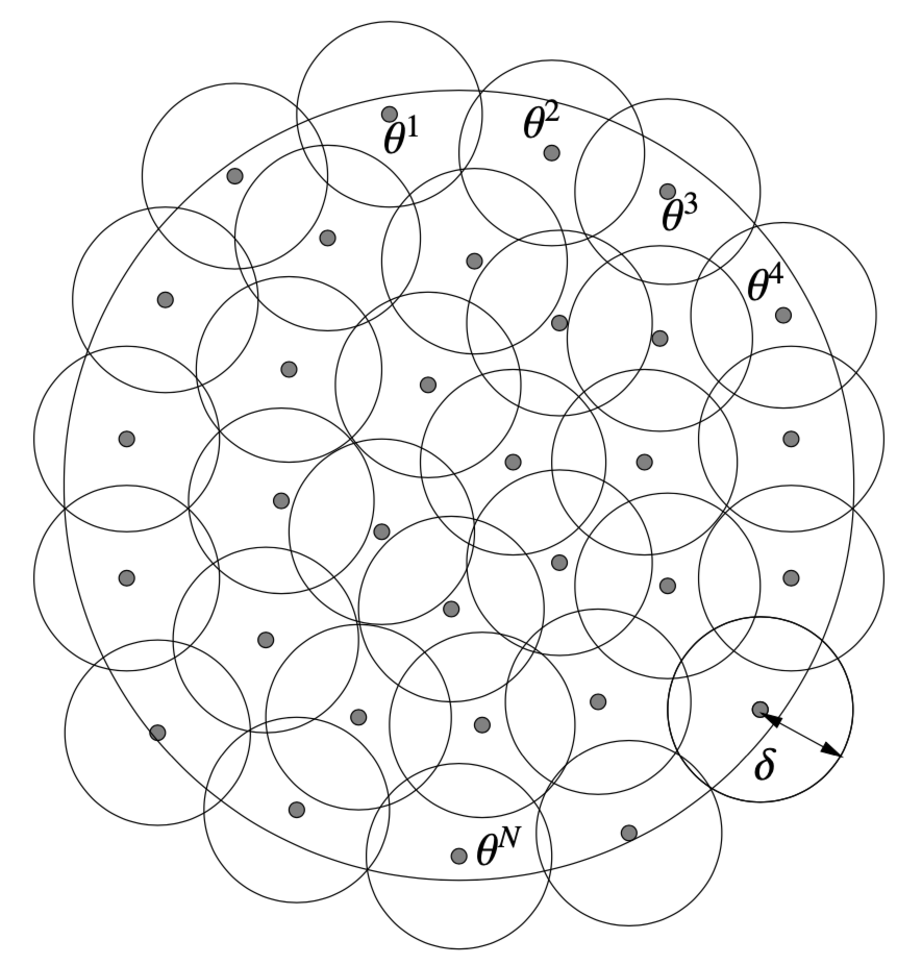
\includegraphics[width=0.45\textwidth]{covering.pdf}
\caption{\it Illustration of a covering using balls of radius $\delta$. The
  entropy is the logarithm of the smallest possible number of balls in such a
  covering. Credit: Chapter 5.1 of \citet{wainwright2019high}.}
\label{fig:covering}
\end{figure}

Seemingly unrelated, but actually connected, is Rademacher complexity. This
itself comes in two flavors. The \emph{empirical Rademacher complexity} based on
a sample $x_1,\dots,x_n$ is the expected largest absolute inner product
achievable with i.i.d.\ Rademacher noise $\sigma_1,\dots,\sigma_n$ (each of 
which take on the value $\pm 1$ with equal probability). To be precise, this is 
defined as   
\[
\Rad(\cF, x_{1:n}) = \E_\sigma \Bigg[ \sup_{f \in \cF} \, \frac{1}{n} \Bigg| 
\sum_{i=1}^n \epsilon_i f(x_i) \Bigg| \Bigg]. 
\]
The expectation above is over $\sigma_1,\dots,\sigma_n$ (as signified by the
subscript notation, $\E_\sigma$), with $x_1,\dots,x_n$ fixed. The
\emph{population Rademacher complexity} is then defined as the expected value of
the empirical Rademacher complexity over i.i.d.\ draws $x_1,\dots,x_n$,
\[
\Rad(\cF) = \E_{x,\sigma} \Bigg[ \sup_{f \in \cF} \, \frac{1}{n} \Bigg| 
\sum_{i=1}^n \epsilon_i f(x_i) \Bigg| \Bigg]. 
\]
To emphasize, the expectation above is over both $\sigma_1,\dots,\sigma_n$ and
$x_1,\dots,x_n$.

A general result connecting these two notions of complexity is called
\emph{Dudley's entropy integral}, which we can state as follows. Denote by
$B_n(\rho)$ the ball in the norm $\|\cdot\|_n$ (the empirical norm based on
$x_1,\dots,x_n$) of radius $\rho>0$ centered at the origin. Then there exists a
constant $c>0$ such that  
\begin{equation}
\label{eq:dudley_integral}
\Rad(\cF \cap B_n(\rho), x_{1:n}) \leq \frac{c}{\sqrt n} \int_0^\rho
\sqrt{\log N(\delta, \cF, \|\cdot\|_n)} \, d \delta.
\end{equation}

% Example 5.24 in Chapter 5.3 of Wainwright (2019)

Entropy and Rademacher complexity are each interesting and important, and have
several applications in probability and nonparametric analysis, but for our
purposes, we can think of them as follows. Entropy arises naturally in a
probabilistic technique known as chaining. This can be used to control
sub-Gaussian processes; in particular, it can be used to bound what is known as
the sub-Gaussian complexity   
\[
\sup_{f \in \cF} \, \Bigg| \frac{1}{n} \sum_{i=1}^n \epsilon_i f(x_i) \Bigg|, 
\]
where $\epsilon_1,\dots,\epsilon_n$ are i.i.d.\ mean zero sub-Gaussian random
variables (to be defined precisely below). We'll see this quantity arising
naturally in our error analysis of smoothing splines, and we'll see the role
entropy plays in Lemma \ref{lem:sg_complexity} below. 

On the other hand, Rademacher complexity appears when using a technique called
symmetrization, and other techniques, to analyze the fluctuations of empirical
averages around their population means. For us, we will see it can be used to
control the difference between the empirical $\|\cdot\|_n$ and population
$\|\cdot\|_2$ norms, with high probability (over the draws of
$x_1,\dots,x_n$). We'll see this in Lemma \ref{lem:norm_coupling} below.     

Lastly, we remark that we are commonly interested in (an upper bound on) how
$\log N(\delta, \cF, \|\cdot\|_n)$ scales with $\delta$, as $\delta \to 0$, and
since we are considering here the empirical norm $\|\cdot\|_n$, we ideally want
log covering number bounds that hold for any arrangement of
$x_1,\dots,x_n$. Observe that this can be upper bounded by $\log N(\delta, \cF, 
\|\cdot\|_\infty)$ where $\|\cdot\|_\infty$ is the sup norm (because
$\|f-g\|_\infty \leq \delta$ implies $\|f-g\|_n \leq \delta$). Table
\ref{tab:entropy} gives entropy rates for a few example function classes of 
interest.  

\begin{table}[tb]
\centering
\renewcommand{\arraystretch}{1.5}
\begin{tabular}{m{3in}|c|c}
Function class $\cF$ & Norm $\|\cdot\|$ & Entropy rate \\ \hline 
$r$-dimensional (e.g., class of natural splines with $r$ knots) with $\diam(\cF,
  \|\cdot\|_n) = \rho$ & $\|\cdot\|_n$ & $r \log(\rho/\delta)$ \\ \hline
% Example 5.8 in Chapter 5.1 of Wainwright (2019)
$L$-Lipschitz functions on $[0,1]^d$ & $\|\cdot\|_\infty$ & $(L/\delta)^d$
  \\ \hline
% Example 5.10 in Chapter 5.1 of Wainwright (2019)
$m$ times weakly differentiable functions on $[0,1]$ such that $\int_0^1 
[D^m f(x)]^2 \, dx \leq L$ and $\|f\|_\infty \leq b$, for an integer $m \geq 1$
& $\|\cdot\|_\infty$ & $(L/\delta)^{1/m} + \log(b/\delta)$ \\ \hline  
\end{tabular}
\caption{\it Entropy rates for some function classes of interest in
  nonparametric analysis.} 
\renewcommand{\arraystretch}{1}
\label{tab:entropy}
\end{table}

\section{Sub-Gaussian random variables}

\emph{Sub-Gaussianity} is a condition that captures some of the key properties
of the Gaussian tail (but at the same time accomodates many distributions that
are not Gaussian).   

A random variable $X$ is said to be sub-Gaussian with mean $\mu$ and
variance proxy $\sigma^2>0$ if   
\[
\E[ e^{t (X - \mu)} ] \leq e^{\sigma^2 t^2 / 2}, \quad \text{for all $t \in
  \R$}. 
\]
This says that the moment generating function of $X$ is dominated by the moment
generating function of $N(\mu, \sigma^2)$ random variable. It turns out that an
equivalent characterization of sub-Gaussianity is that
\[
\P(|X-\mu| \geq t) \leq c \, \P(|Z| \geq t), \quad \text{for all $t \in \R$},
\]
for some constant $c>0$, where $Z \sim N(0,1)$. This is perhaps more intuitive
and explains the name ``sub-Gaussian'': the tails must decay at least as fast as
that of the Gaussian distribution. 

% Theorem 2.16 (II) in Section 2.1 of Wainwright (2019)

Here are some examples of sub-Gaussian random variables.

\begin{itemize}
\item A $N(\mu, \sigma^2)$ random variable. 
\item A bounded random variable. Thus, e.g., Rademacher, Bernoulli, and binomial   
  random variables are all sub-Gaussian.
\item A random variable $X$ for which all even moments exist and satisfy  
\[
\E[X^{2k}] \leq \frac{(2k)!}{2^k k!} \theta^{2k}, \quad \text{for all
  $k=1,2,3,\dots$},
\]
for some parameter $\theta \geq 0$. In fact this moment condition is equivalent
to sub-Gaussianity.   
% Theorem 2.6 (III) in Section 2.1 of Wainwright (2019)
\end{itemize}

An example of a random variable that is not sub-Gaussian is a Poisson random
variable with any mean $\mu$ (this is instead \emph{sub-exponential}, which is a 
weaker condition).

Next we give several useful bounds for sub-Gaussian random variables. We won't
need all of them in our main analysis, but they are simple and important
nonetheless (and we may use them in later lectures).  

\subsection{Tail bound for averages}

An important fact about sub-Gaussian random variables is that they admit a 
Bernstein-type tail bound: if $X_i$, $i=1,\dots,n$ are independent sub-Gaussian
random variables, with each $X_i$ having mean zero and variance proxy
$\sigma_i^2$, then for all $t>0$,    
\begin{equation}
\label{eq:sg_average}
\P(\bar{X}_n \geq t) \leq \exp \bigg( \frac{-nt^2}{
    \frac{2}{n}\sum_{i=1}^n \sigma_i^2} \bigg),
\end{equation}
where \smash{$\bar{X}_n = \frac{1}{n} \sum_{i=1}^n X_i$}. We can also get a
two-sided bound where we multiply right-hand side above by 2 (since $X$ is mean
zero sub-Gaussian with variance proxy $\sigma^2$ if and only if $-X$ is).    

\subsection{Tail bound for maxima}

Another useful fact about sub-Gaussian random variables is that maximum of a
large number of them sharply concentrates: if $X_i$, $i=1,\dots,n$ are sub-Gaussian
random variables, which need not be independent, and each $X_i$ has mean zero
and variance proxy $\sigma^2$, then for all $t>0$,    
\begin{equation}
\label{eq:sg_max_prob}
\P \Big(\max_{i=1,\dots,n} \, X_i \geq \sigma \sqrt{2 (\log n + t)} \Big) \leq
e^{-t}.  
\end{equation}
It also holds that 
\begin{equation}
\label{eq:sg_max_exp}
\E \Big[ \max_{i=1,\dots,n} \, X_i \Big] \leq \sigma \sqrt{2 \log n}.
\end{equation}

\subsection{Tail bound for quadratic forms}

A last useful fact we will cite about sub-Gaussian random variables concerns
tail concentration for quadratic forms: if $X_i$, $i=1,\dots,n$ are independent
sub-Gaussian random variables, with each having mean zero and variance proxy 
$\sigma^2$, then for any positive semidefinite matrix $Q \in \R^{n \times n}$
and all $t>0$,    
\begin{equation}
\label{eq:sg_quadratic}
\P\Big( X^\T Q X \geq \sigma^2 \big[ \tr(Q) + 2 \|Q\|_F {\sqrt t} + 2 
\|Q\|_{\mathrm{op}} \, t \big] \Big) \leq e^{-t},
\end{equation}
where $X = (X_1,\dots,X_n) \in \R^n$ is the vector of sub-Gaussian variates, so 
that \smash{$ X^\T Q X = \sum_{i,j=1}^n Q_{ij} X_i X_j$}, and \smash{$\|Q\|_F, 
\|Q\|_{\mathrm{op}}$} denote the Frobenius and operator norms of $Q$, 
respectively. The result we are stating here is from \citet{hsu2012tail}, which
is similar to the Hanson-Wright inequality (but has simple explicit constants).       
Note in particular that when \smash{$Q = \frac{1}{n} I$}, we get
\begin{equation}
\label{eq:sg_sum_squares}
\P\bigg( \frac{1}{n} \sum_{i=1}^n X_i^2 \geq \sigma^2 \big[ 1 + 2 \sqrt{t/n} +
2t/n \big] \bigg) \leq e^{-t}.  
\end{equation}

\section{Sub-Gaussian complexity}

We now present the first of two powerful tools we'll use from empirical process
theory. It will be used to control the supremum of a sub-Gaussian process,
indexed by functions $f \in \cF$. We call such a quantity   
\[
\sup_{f \in \cF} \, |\langle \epsilon, f \rangle_n|
\]
the \emph{sub-Gaussian complexity} associated with $\cF$, based on a sample 
$x_1,\dots,x_n$, used to define the empirical inner product. The next result
controls this quantity, uniformly over all $x_1,\dots,x_n$. 

\begin{lemma}[Adapted from Lemma 8.4 of \citealt{vandegeer2000empirical}] 
\label{lem:sg_complexity}
Let $\epsilon_i$, $i=1,\ldots,n$ denote independent sub-Gaussian random
variables, each having mean zero variance proxy $\sigma^2$. Assume that there
exist constants $0<w<2$ and $C>0$ such that for some fixed $x_1,\dots,x_n$
(which define the empirical norm $\|\cdot\|_n$), 
\begin{equation}
\label{eq:entropy_bd}
\log N\big(\delta, \cF, \|\cdot\|_n \big) \leq C \delta^{-w},
\end{equation}
for sufficiently small $\delta>0$. Then for any fixed $\rho>0$, there exist
constants $n_0,c_0,c_1>0$, depending only on $\sigma,\rho,C,w$, such that for
all $n \geq n_0$ and $\gamma \geq c_0$,  
\begin{equation}
\label{eq:sg_complexity}
\sup_{f \in \cF \cap B_n(\rho)} \, \frac{|\langle \epsilon, f
  \rangle_n|}{\|f\|_n^{1-w/2}} \leq \frac{\gamma}{\sqrt n},  
\end{equation}
with probability at least $1 - \exp(-c_1\gamma^2)$.
\end{lemma}

To get a sense of what the result in the lemma gives us, let's rewrite the
conclusion in \eqref{eq:sg_complexity} a little differently: it says that
uniformly over all $f \in \cF$ with $\|f\|_n \leq \rho$, we have  
\[
|\langle \epsilon, f \rangle_n| \leq \gamma \|f\|_n \frac{\|f\|_n^{-w/2}}
{\sqrt n}, 
\]
with high probability. Now think about what a simple application of
Cauchy-Schwarz would give us: 
\[
|\langle \epsilon, f \rangle_n| \leq \|\epsilon\|_n \|f\|_n \leq c \|f\|_n, 
\]
where the second inequality holds with high probability, for some constant  
$c>0$, by the result \eqref{eq:sg_sum_squares} for a quadratic form of
sub-Gaussians. If we ignore the leading factors of $\gamma, c$, then we see that
the second-to-last display is better than the last display when   
\[
\frac{\|f\|_n^{-w/2}}{\sqrt n} \leq 1 \iff \|f\|_n \geq n^{-1/w}.
\]
That is, except for functions $f$ of really small empirical norm, we improve on
Cauchy-Schwarz, and dramatically so when $f$ is of larger empirical norm. For
example, when \smash{$\|f\|_n = n^{-1/(2+w)}$} (this is not an arbitrarily
chosen rate, you'll see why we're interested in this a bit later, when we do the
error analyis), then the ``speedup'' we get from \eqref{eq:sg_complexity} is:   
\[
\frac{\|f\|_n^{-w/2}}{\sqrt n} = n^{-1/(2+w)}.
\]

\section{Empirical and population norm coupling}

This section states the second of two powerful tools we'll use from empirical 
process theory. It will be used to control the supremum of difference between
empirical and population norms, over all $f \in \cF$ for some function class
$\cF$. Strictly speaking it won't be needed for the result in the main analysis,
which bounds the empirical norm error, but we'll use it in the corollary given
at the end, on the population norm error. 

We need to cover a few more preliminary concepts before stating the result. We
say that $\cF$ is \emph{star-shaped} if $f \in \cF$ implies $\alpha f \in \cF$
for all $\alpha \in [0,1]$. We say that $\cF$ is \emph{$b$-bounded} if $\cF
\subseteq B_\infty(b)$, the sup norm ball of radius $b$. Lastly and most
importantly, we will introduce \emph{localized} notions of Rademacher
complexity. For $\delta>0$, we define the localized empirical Rademacher
complexity by    
\[
\hat{R}_n(\delta) = \Rad(\cF \cap B_n(\delta), x_{1:n}) 
= \E_\sigma \Bigg[ \sup_{f \in \cF \cap B_n(\delta)} \, \frac{1}{n} \Bigg|  
\sum_{i=1}^n \epsilon_i f(x_i) \Bigg| \Bigg],
\]
where $B_n(\delta)$ is the empirical norm ball of radius $\delta$. Similarly, we
define the localized population Rademacher complexity by   
\[
R_n(\delta) = \Rad(\cF \cap B_2(\delta))
= \E_{x,\sigma} \Bigg[ \sup_{f \in \cF \cap B_2(\delta)} \, \frac{1}{n} \Bigg|  
\sum_{i=1}^n \epsilon_i f(x_i) \Bigg| \Bigg],
\]
where $B_2(\delta)$ is the population norm ball of radius $\delta$. We are now
ready to state the result, which we informally call a ``coupling'' between
empirical and population norms.

\begin{lemma}[Adapted from Theorem 14.1 and Proposition 14.25 of
  \citealt{wainwright2019high}]  
\label{lem:norm_coupling}
Let $\cF$ be a star-shaped and $b$-uniformly bounded class of functions for some 
$b>0$. Denote by \smash{$\hat\delta_n$} the smallest positive solution to 
\[
\hat{R}_n(\delta) \leq \delta^2 / b.
\]
and denote by $\delta_n$ the smallest positive solution to
\[
R_n(\delta) \leq \delta^2 / b.
\]
Assume $n\delta_n^2 \geq c_0 \log\log(1/\delta_n)$ for a constant $c_0>0$. 
Then there exist constants $a,m_1,m_2,c_1>0$ such that with probability at
least $1 - a \exp(-n \delta_n^2 / (c_0 b))$, both of the following two
statements hold:
\begin{gather}
\label{eq:radius_coupling}
m_1 \delta_n \leq \hat\delta_n \leq m_2 \delta_n, \\
\label{eq:norm_coupling}
\Big| \|f\|_n - \|f\|_2 \Big| \leq c_1 \delta_n, \quad \text{for all $f \in
  \cF$}. 
\end{gather}
\end{lemma}

The punchline in the lemma is really \eqref{eq:norm_coupling}, which says that
the empirical and population norms are uniformly close over all $f \in
\cF$. In traditional nonparametric applications, we should think of $\delta_n$
as being small, scaling as $n^{-\alpha}$ for some $\alpha <  1/2$, in which case
the uniform coupling \eqref{eq:norm_coupling} gives us a strong result. Note
that for such a scaling on $\delta_n$, we will meet the required assumption
$n\delta_n^2 \geq c_0 \log\log(1/\delta_n)$, since   
\[
n\delta_n^2 = n^{1-2\alpha} \quad \text{and} \quad\log\log(1/\delta_n) = \alpha
\log\log n.
\]

Backing up somewhat, we call $\delta_n$ the \emph{population critical radius} of
$\cF$, and \smash{$\hat\delta_n$} the \emph{empirical critical radius} of
$\cF$. The reason for introducing the latter (which, note, is a random quantity)
is that it can be sometimes easier to bound, using Dudley's entropy integral
\eqref{eq:dudley_integral}. Then, the result in \eqref{eq:radius_coupling}
provides the link between the two---it says that the scaling of the empirical
critical radius determines that of the population critical radius, with high
probability.    

The following calculation demonstrates this connection, and will be useful later
on.

\begin{lemma}
\label{lem:critical_rad}
Assume that $\cF$ satisfies the entropy bound \eqref{eq:entropy_bd} for
sufficiently small $\delta>0$ and all $x_1,\dots,x_n$, where $0<w<2$ and $C>0$
are constants. Then the empirical critical radius of $\cF$ satisfies
\smash{$\hat\delta_n \leq c_1 n^{-1/(2+w)}$} for a constant $c_1>0$. By
\eqref{eq:radius_coupling}, assuming further that $\cF$ is star-shaped and
$b$-bounded, we hence also have \smash{$\delta_n \leq c_2 n^{-1/(2+w)}$} with
probability at least \smash{$1 - \exp(-c_3 n^{2/(2+w)})$}, for constants
$c_2,c_3>0$.      
\end{lemma}

\begin{proof}
By \eqref{eq:dudley_integral}, we have
\begin{align*}
\Rad(\cF \cap B_n(\delta), x_{1:n}) &\leq \frac{c}{\sqrt n} \int_0^\delta 
\sqrt{\log N(t, \cF, \|\cdot\|_n)} \, dt \\
&\leq \frac{{\sqrt C} c}{\sqrt n} \int_0^\delta t^{-w/2} \, dt \\ 
&= \frac{c}{\sqrt n} \delta^{1-w/2}.
\end{align*}
In the second line we applied the entropy bound \eqref{eq:entropy_bd}, and in
the third we simply computed the integral, redefining the constant $c>0$ as
necessary. The smallest positive solution \smash{$\hat\delta_n$} to
\smash{$\hat{R}_n(\delta) \leq \delta^2/b$} can therefore by upper bounded by
solving 
\[
\frac{c}{\sqrt n} \delta^{1-w/2} = \delta^2 / b \iff \delta^{1+w/2} =
\frac{(c/b)}{\sqrt n}, 
\]
which gives \smash{$\hat\delta_n \leq c_1 n^{-1/(2+w)}$} for a constant
$c_1>0$. The statement for $\delta_n$ is given by applying
\eqref{eq:radius_coupling}.   
\end{proof}

\section{Main analysis} 

Euipped with these tools, we are now ready to dive into the main analysis. In
this section, we will prove the following theorem.   

\begin{theorem}
\label{thm:main}
Let $(x_i,y_i)$, $i=1,\dots,n$ be i.i.d.\ satisfying \eqref{eq:model}, where
each $\epsilon_i$ is sub-Gaussian with mean zero and variance proxy
$\sigma^2>0$, each $x_i \sim Q$, an arbitrary continuous distribution supported
on $[0,1]$, and each $x_i \indep \epsilon_i$. Let $J$ be a seminorm acting on
$m$ times weakly differentiable functions, and assume that the following
conditions hold for an integer $k \geq 0$, and constants $0<w<2$ and $M,C>0$: 
\begin{enumerate}[label=A\arabic*.]
\item the null space of $J$ consists of $k\th$ order polynomials;
\item $\sup_{x \in [0,1]} D^m f (x) - \inf_{x \in [0,1]} D^m f(t) \leq M$ for
  all functions $f \in B_J(1)$;
\item $\cF = B_J(1) \cap B_\infty(1)$ satisfies the entropy bound $\log
  N(\delta, \cF, \|\cdot\|_\infty) \leq C \delta^{-w}$, for small enough
  $\delta>0$. 
\end{enumerate}
To be clear, here we denote by $B_J(1)$ the unit ball in $J$, and by
$B_\infty(1)$ the unit ball in sup norm. Finally, assume that the underlying
regression function satisfies $1 \leq J(f_0) < \infty$.  

Then there exists constants $c_0,c_1,c_2,c,n_0>0$ that depend only on   
$\sigma,k,M,C,w$ such that for all $n \geq n_0$ and $\gamma \geq c_0$, the 
following holds. Fix any fixed exponent $v > 2w/(2+w)$. Any solution
\smash{$\hf$} to the problem  
\begin{equation}
\label{eq:variational_opt_v}
\minimize_f \; \frac{1}{n} \sum_{i=1}^n (y_i - f(x_i))^2 + \lambda J^v(f), 
\end{equation}
with tuning parameter value \smash{$\gamma n^{-2/(2+w)} J(f_0)^{2w/(2+w) - v}
  \leq \lambda \leq \sigma^2 J(f_0)^{2-v}$}, satisfies     
\begin{equation}
\label{eq:error_bd1}
\|\hf - f_0\|_n^2 \leq 2 \lambda J^v(f_0) \quad \text{and} \quad J(\hf) \leq c
J(f_0), 
\end{equation}
with probability at least $1 - \exp(-c_1\gamma) - \exp(-c_2n)$. 

In particular, for \smash{$\lambda = \gamma n^{-2/(2+w)} J(f_0)^{2w/(2+w) -
    v}$}, it holds that  
\begin{equation}
\label{eq:error_bd2}
\|\hf - f_0\|_n^2 \leq 2 \gamma n^{-2/(2+w)} J(f_0)^{2w/(2+w)},
\end{equation}
with the same probability.
\end{theorem}

The proof is similar to that for Theorem 10.2 in \citet{vandegeer2000empirical},
except we make all the statements finite-sample, following a development similar
to that in Theorem 1 of \citet{sadhanala2019additive}.   

\subsection{Remarks} 

Before delivering the proof in the next subsection, we make several remarks.  

\begin{itemize}
\item The proof for the estimator defined by the analogous constrained problem 
  \[
  \minimize_f \; \sum_{i=1}^n (y_i - f(x_i))^2 \;\; \st \;\; J(f) \leq t,
  \]
  is actually much simpler. (We'll see this when we analyze the lasso, in the
  next lecture.) But penalized estimators are more common in practice. 

\item Theorem \ref{thm:main} is not the ``pinnacle'' of what can be achieved
  with this type of analysis, it's just supposed to be a (relatively simple and
  clean) example of what can be achieved. For example, we could also use similar
  techniques to analyze multivariate estimators, such as thin plate splines (in 
  the supercritical regime $2m > d$; see Chapter 10.3 of
  \citet{vandegeer2000empirical}) and RKHS regression (see Chapter 13.4 of
  \citealt{wainwright2019high}).    

\item Another important generalization that is important to mention is the
  following. We can extend the result in Theorem \ref{thm:main} to an estimator
  that is defined by minimization over a set $\cS$:
  \[
  \minimize_{f \in \cS} \; \frac{1}{n} \sum_{i=1}^n (y_i - f(x_i))^2 + \lambda
  J^v(f),  
  \]
  for a set of functions $\cS$ of our choosing. The set $\cS$ need not contain
  any solutions to the unrestricted problem in \eqref{eq:variational_opt_v}. It 
  need not contain the true regression function $f_0$. It's just something we
  choose for (say) computational convenience. For example, we may choose $\cS$
  to be a space of splines, since splines are nice to work with
  computationally---and again, we do not need it to be true that $\cS$ actually
  contains a solution in \eqref{eq:variational_opt_v}. Then an extension of the
  analysis you'll see in the coming subsection will produce a guarantee of the
  form
  \[
  \|\hf - f_0\|_n^2 \leq \inf_{\bar{f} \in \cS} \, \Big( \|\bar{f} - f_0\|_n^2
  + c \lambda \max\{ J(f_0),  J(\bar{f}) \}^v \Big),
  \]
  with high probability (for some constant $c>0$). This is often called an 
  \emph{oracle inequality}. The first term in the above \smash{$\|\bar{f} -
    f_0\|_n^2$} can be made small by ensuring that $\cS$ is chosen to have good
  approximation guarantees over $\{ f : [0,1] \to \R \,:\, J(f) < \infty\}$. For
  example, this is true, with respect to various seminorms $J$, if we choose
  $\cS$ to be a space of splines with suitably chosen knots. In such cases, the 
  approximation error term \smash{$\|\bar{f} - f_0\|_n^2$} will be of much
  smaller order than the second term \smash{$2 \lambda \max\{ J(f_0), J(\bar{f})
    \}^v$}, which will scale as \smash{$n^{-2/(2+w)}$} when $J(f_0) \asymp 1$
  (as seen in \eqref{eq:error_bd2}). This is very useful because it means that
  we can use splines to approximately solve \eqref{eq:variational_opt}
  (regardless of whether or not splines actually solve
  \eqref{eq:variational_opt} or not) and we will not incur any loss in the 
  statistical error rate. We will not cover the details, but refer to Theorem 1
  and Corollary 1 in \citet{sadhanala2019additive} for an example of such a
  result.       

  (We'll also derive explicit oracle inequalities in the next lecture on the
  lasso.)  

\item The rate in \eqref{eq:error_bd2} is minimax optimal. This can be shown
  using Fano's inequality along with a construction that leverages a concept 
  complementary to covering numbers (metric entropy) called \emph{packing
    numbers}. See Theorem 4 in \citet{sadhanala2019additive} for details.  
\end{itemize}

\subsection{Proof}

We now prove Theorem \ref{thm:main}. By the exact same arguments used earlier to
produce \eqref{eq:basic_ineq} from problem \eqref{eq:variational_opt}, we have
for our current problem \eqref{eq:variational_opt_v} the basic inequality     
\begin{equation}
\label{eq:basic_ineq_v1}
\|\hf - f_0\|_n^2 \leq 2 \langle \epsilon, \hf-f_0 \rangle_n + \lambda (J^v(f_0)
- J^v(\hf)), 
\end{equation} 
We break down the rest of the proof into parts, henceforth abbreviating
\smash{${\hat J} = J(\hf)$} and $J_0 = J(f_0)$.     

\paragraph{Localization.}

In this part, we prove that \smash{$\|\hf - f_0\|_n$} is bounded. This is
important because it will be enable us to apply Lemma
\ref{lem:sg_complexity}. By the sub-Gaussian tail bound in
\eqref{eq:sg_sum_squares}, taking $t=n$, we know that    
\[
\|\epsilon\|_n^2 \leq 5\sigma^2,
\]
on an event $\Omega_1$ with probability at least $1-\exp(-n)$. Hence, returning
to  \eqref{eq:basic_ineq_v1}, using Cauchy-Schwarz and the above bound, we have
on $\Omega_1$, 
\begin{align*}
\|\hf-f_0\|_n^2 &\leq 2{\sqrt 5}\sigma \|\hf-f_0\|_n + 
  \lambda (J_0^v - {\hat  J}^v) \\  
&\leq 2{\sqrt 5}\sigma \|\hf-f_0\|_n + \lambda J_0^v.
\end{align*}
This is a quadratic inequality of the form $x^2 \leq bx + c$ in \smash{$x=\|\hf
  - f_0\|_n$}, so we can upper bound $x$ by the larger of the two roots,
\smash{$x \leq (b+\sqrt{b^2+4c})/2 \leq b+\sqrt{c}$}, which gives, on
$\Omega_1$, 
\begin{align}
\nonumber
\|\hf-f_0\|_n &\leq 2{\sqrt 5}\sigma + \sqrt{\lambda J_0^v} \\
\label{eq:localization}
&\leq (2{\sqrt 5} + 1) \sigma J_0,
\end{align}
where in the second line we use $J_0\geq 1$ and $\lambda \leq \sigma^2 
J_0^{2-v}$. This completes the desired ``localization'' step.     

\paragraph{Bounding the sub-Gaussian complexity.}

In this part, we focus on bounding the first-term on the right-hand side in 
\eqref{eq:basic_ineq_v1} using a sub-Gaussian complexity argument. The idea is
the same as what we described in the introduction. Let
\[
g = \frac{\hf-f_0}{({\hat J} + J_0)}.
\]
By construction, we have $J(g) \leq 1$. Further, from \eqref{eq:localization},
we have $\|g\|_n \leq (2{\sqrt 5} + 1) \sigma$ on $\Omega_1$.  

We would like to apply Lemma \ref{lem:sg_complexity} in order to bound $\langle 
\epsilon, g \rangle_n$, but we need one more step first. Assumption A3 in the
theorem statement is about an entropy condition for the class $\cF = B_J(1) \cap
B_\infty(1)$. But at present, we do not know that $g$ is bounded in sup norm,
only in empirical norm. An argument (whose details we do not give) involving
orthogonalization with respect to functions in the null space of $J$, which
recall are polynomials of degree $k$, can be used to show that for constants
$q_1,q_2,c_2>0$, 
\[
\|g\|_\infty \leq q_1 J(g) + q_2 \|g\|_n,
\]
on an event $\Omega_2$ with probability at least $1-\exp(-c_2 n)$. See Lemma 7
(and Lemmas 4, 5, and 6 leading up to it) in \citet{sadhanala2019additive}. We
note that this is why we need Assumptions A1 and A2, and the assumption that the 
input distribution $Q$ is continous.   

Thus, rescaling the definition of $g$ by a constant $c>0$ as needed, 
\[
g = \frac{\hf-f_0}{c({\hat J} + J_0)},
\]
we have $J(g) \leq 1$ and $\|g\|_\infty \leq 1$ on $\Omega_1 \cap
\Omega_2$. Lemma \ref{lem:sg_complexity} then says that for constants
$c_0,c_1>0$ and all $\gamma \geq c_0$ and sufficiently large $n$,     
\[
\langle \epsilon, g \rangle_n \leq \frac{\gamma \|g\|_n^{1-w/2}}{\sqrt n} 
\]
on an event $\Omega_1 \cap \Omega_2 \cap \Omega_3$ with probability at least 
with probability at least $1 - \exp(-c_1\gamma^2) - \exp(-c_2n)$. Plugging this 
into the right-hand side of \eqref{eq:basic_ineq_v1} gives 
\begin{align}
\nonumber
\|\hf - f_0\|_n^2 &\leq 2c \gamma \frac{({\hat J} + J_0)}{\sqrt n}
 \|g\|_n^{1-w/2} + \lambda (J_0^v - {\hat J}^v) \\ 
\label{eq:basic_ineq_v2}
&= 2c \gamma \frac{({\hat J} + J_0)^{w/2}}{\sqrt n} \|\hf-f_0\|_n^{1-w/2} +
  \lambda (J_0^v - {\hat J}^v), 
\end{align} 
on the event $\Omega = \Omega_1 \cap \Omega_2 \cap \Omega_3$, where we have
redefined the constant $c$ as needed.

\paragraph{Transforming to squared empirical norm.} 

The next part is to transform \eqref{eq:basic_ineq_v2} so that we remove the
fractional exponent on the empirical norm error term \smash{$\|\hf-f_0\|_n$},
and end up with only squared empirical norm terms. First, we use the following
inequality that holds for any $a,b \geq 0$, and any $w$,    
\[
a b^{1-w/2} \leq a^{1/(1+w/2)} b + a^{2/(1+w/2)}.
\]
Applying this to the first term on the right-hand side in
\eqref{eq:basic_ineq_v2} with \smash{$a = ({\hat J} +  J_0)^{w/2} / {\sqrt n}$}
and \smash{$b = \|\hf-f_0\|_n$}, and abbreviating \smash{$r_n = n^{-1/(2+w)}$},
yields 
\[
\|\hf - f_0\|_n^2 \leq 2c \gamma r_n ({\hat J} + J_0)^{w/(2+w)} \|\hf-f_0\|_n +
2c \gamma r_n^2 ({\hat J} + J_0)^{2w/(2+w)} + \lambda (J_0^v - {\hat J}^v), 
\]
on $\Omega$. At this point, we could recognize the above as a quadratic
of the form $x^2 \leq bx + c$ in \smash{$x = \|\hf-f_0\|_n$}, and proceed as we
did in the localization step, but we take a different approach that leads to a
slightly sharper dependence on various problem parameters. We apply $2ab \leq
a^2+b^2$ to the first term on the right-hand side of the above display, with
\smash{$a = \sqrt{2}c \gamma r_n ({\hat J} +  J_0)^{w/(2+w)}$} and \smash{$b =
  \|\hf-f_0\|_n/\sqrt{2}$}, which yields          
\[
\|\hf - f_0\|_n^2 \leq \frac{1}{2}\|\hf - f_0\|_n^2 + \gamma r_n^2 ({\hat J} +
J_0)^{2w/(2+w)} + \lambda (J_0^v - {\hat J}^v),   
\]
on $\Omega$, where we have redefined $\gamma$ as needed. We have been careful to 
end up with a factor of the squared empirical norm on the right-hand side with a
leading constant less than 1. Subtracting this term \smash{$\frac{1}{2}
\|\hf-f_0\|_n^2$} to the left-hand side gives, on $\Omega$,
\begin{equation}
\label{eq:basic_ineq_v3}
\frac{1}{2} \|\hf - f_0\|_n^2 \leq \gamma r_n^2 ({\hat J} + J_0)^{2w/(2+w)} +
\lambda (J_0^v - {\hat J}^v).
\end{equation}

\paragraph{Bounding the achieved penalty term.}

The next part is to bound the achieved penalty term \smash{$\hat J$}. Starting
from \eqref{eq:basic_ineq_v3}, we can simply lower bound the left-hand side by
zero, and rearrange, yielding 
\[
{\hat J}^v \leq \frac{\gamma r_n^2}{\lambda} ({\hat J} + J_0)^{2w/(2+w)} +
J_0^v, 
\]
on $\Omega$. Suppose \smash{$\hat J > 2J_0$}. Then upper bounding the first term
on right-hand side above,
\[
{\hat J}^v \leq c \frac{\gamma r_n^2}{\lambda} {\hat J}^{2w/(2+w)} +
\frac{1}{2}{\hat J}^v, 
\]
on $\Omega$, for a constant $c>0$. Subtracting \smash{$\frac{1}{2}{\hat J}^v$}
to the left-hand side, we learn that provided \smash{$\lambda \geq \gamma
  r_n^2$},  
\begin{equation}
\label{eq:penalty_bd}
\frac{1}{2}{\hat J}^v \leq c {\hat J}^{2w/(2+w)},
\end{equation}
on $\Omega$. Since $v > 2w/(2+w)$, this means that \smash{$\hat J \leq c$} on
$\Omega$, where we redefine the constant $c$ as necessary. Recall that this was
established in the case \smash{$\hat J > 2J_0$}.  Hence, altogether, we learn
that \smash{$\hat J \leq 2J_0+c \leq cJ_0$} on $\Omega$, redefining $c$ once
again as needed.     

\paragraph{The home stretch: choosing $\lambda$.}

Returning to \eqref{eq:basic_ineq_v3}, and using our penalty bound from
\eqref{eq:penalty_bd}, we have 
\[
\|\hf - f_0\|_n^2 \leq \gamma r_n^2 J_0^{2w/(2+w)} + \lambda J_0^v,
\]
on $\Omega$, redefining $\gamma$ as needed. Choosing $\lambda \geq \gamma r_n^2
J_0^{2w/(2+w)   - v}$ establishes \eqref{eq:error_bd1}, and completes the proof.          

\subsection{Corollary: population error}

Using the coupling between empirical and population norms, we can also bound the
population error as a corollary to Theorem \ref{thm:main}.

\begin{corollary}
\label{cor:main}
Under the same conditions and notation as in Theorem \ref{thm:main}, there
exists constants $c_3,c_4 > 0$ such that for all $n \geq n_0$ and $\gamma \geq
c_0$, 
\begin{equation}
\label{eq:error_bd3}
\|\hf - f_0\|_2^2 \leq 4 \lambda J^v(f_0) + c_3 n^{-2/(2+w)} J^2(f_0),
\end{equation}
with probability at least \smash{$1 - \exp(-c_1\gamma) - \exp(-c_4
  n^{2/(2+w)})$}.  

\end{corollary}

\begin{proof}
Let \smash{$g = (\hf - f_0)/((c+1) J_0)$}. Then, as in the proof of Theorem
\ref{thm:main}, we have $J(g) \leq 1$ and $\|g\|_\infty \leq b$ for a constant
$b>0$, on the event $\Omega$. By Lemma \ref{lem:critical_rad} applied to $\cF = 
B_J(1) \cap B_\infty(b)$, the population critical radius satisfies
\smash{$\delta_n \leq c_3 n^{-1/(2+w)}$} with probability at least \smash{$1 -  
  \exp(-c_1\gamma) - \exp(-c_2n) - \exp(-c_4 n^{2/(2+w)})$}, for constants 
$c_3,c_4>0$. Applying Lemma \ref{lem:norm_coupling}---specifically, applying
\eqref{eq:norm_coupling} to $g$, we see that  
\[
\|\hf - f_0\|_2 \leq \|\hf - f_0\|_n + c_3 n^{-1/(2+w)} J_0,
\]
with probability at least \smash{$1 - \exp(-c_1\gamma) - \exp(-c_2n) - \exp(-q_2
  n^{2/(2+w)})$}, where we adjust $c_3$ as necessary. The result in
\eqref{eq:error_bd3} follows by squaring both sides in the above display, using
\eqref{eq:error_bd1}, and adjusting $c_3,c_4$ once again as needed.  
\end{proof}

A remark: choosing \smash{$\lambda = \gamma n^{-2/(2+w)} J(f_0)^{2w/(2+w) -
    v}$}, we see from \eqref{eq:error_bd3} that when $J(f_0) \asymp 1$ we are
able to bound the population error at the same rate \smash{$n^{-2/(2+w)}$} as
the empirical error. But when $J(f_0)$ is growing with $n$, the population
error rate established by the above corollary is worse. This is likely an
artifact of the proof strategy.  

\subsection{Corollary: smoothing splines}

Finally, we apply Theorem \ref{thm:main} and Corollary \ref{thm:main} to
smoothing splines, where \smash{$J(f) = \int_0^1 (D^m f)^2(x) \, dx$}, in order 
to get the following result.  

\begin{corollary}
\label{cor:ss}
Let $(x_i,y_i)$, $i=1,\dots,n$ be i.i.d.\ satisfying \eqref{eq:model}, where
each $\epsilon_i$ is sub-Gaussian with mean zero and variance proxy
$\sigma^2>0$, each $x_i \sim Q$, an arbitrary continuous distribution supported
on $[0,1]$, and each $x_i \indep \epsilon_i$. Fix an integer $m \geq 1$ and
assume that the underlying regression function satisfies  
\[
1 \leq  J_0^2 = \int_0^1 (D^m f_0)^2(x) \, dx < \infty.
\]
Then there exists constants $c_0,c_1,c_2,c_3,c_4,c,n_0>0$ that depend only on     
$\sigma,m$ such that for all $n \geq n_0$ and $\gamma \geq c_0$, the
smoothing spline estimator \smash{$\hf$}, defined by solving
\[
\minimize_f \; \frac{1}{n} \sum_{i=1}^n (y_i - f(x_i))^2 + \lambda \int_0^1 (D^m
f)^2(x) \, dx, 
\]
for any tuning parameter value \smash{$\gamma n^{-2m/(2m+1)} J_0^{-4m/(2m+1)}
  \lambda \leq \sigma^2$}, satisfies       
\[
\|\hf - f_0\|_n^2 \leq 2 \lambda J_0^2\quad \text{and} \quad 
\int_0^1 (D^m \hf)^2(x) \, dx \leq c J_0^2, 
\]
with probability at least $p_n = 1 - \exp(-c_1\gamma) - \exp(-c_2n)$, and
\[
\|\hf - f_0\|_2^2 \leq 4 \lambda J_0^2 + c_3 n^{-2m/(2m+1)} J_0^2,
\]
with probability at least \smash{$q_n = 1 - \exp(-c_1\gamma) - \exp(-c_4 
  n^{2m/(2m+1)})$}. In particular, for a choice of tuning parameter
\smash{$\lambda = \gamma n^{-2m/(2m+1)} J_0^{-4m/(2m+1)}$}, it holds that  
\[
\|\hf - f_0\|_n^2 \leq 2 \gamma n^{-2m/(2m+1)} J_0^{2/(2m+1)},  
\quad \text{and}  \quad
\|\hf - f_0\|_2^2 \leq n^{-2m/(2m+1)} (4 \gamma J_0^{2/(2m+1)} + c_3 J_0^2), 
\]
with the same probabilities as above: $p_n$ and $q_n$, respectively.
\end{corollary}

\begin{proof}
We must simply check the conditions A1--A3 in Theorem \ref{thm:main} for the
choice \smash{$J(f) = \int_0^1 (D^m f)^2(x) \, dx$}. It is straightforward to
see that A1 and A2 are satisfied with $k=m-1$. The condition A3 is satisfied for
$w=1/m$, as cited in Table \ref{tab:entropy}, which is a result due to
\citet{birman1967piecewise}. The rest is just given by reading off the results
of Theorem \ref{thm:main} and Corollary \ref{cor:main} for $w=1/m$.  
\end{proof}

\bibliographystyle{plainnat}
\bibliography{../../common/ryantibs.bib}

\end{document}
